\documentclass[11pt]{article}
\usepackage[utf8]{inputenc}
\usepackage[T1]{fontenc}
\usepackage[spanish,es-tabla]{babel} % idiomas (uno o varios)

\usepackage[left = 2.25cm, right = 2.25cm, top=1.5cm, bottom = 1.5cm]{geometry}
\usepackage{mathtools} % símbolos extensibles (contiene amsmath)
\usepackage{amssymb} % símbolos matemáticos
\usepackage{mathrsfs} % para usar \mathscr{}
\usepackage{physics} % notación de Dirac
\usepackage{tensor} % índices en cualquier lado

\usepackage{booktabs} % tablas
\usepackage[bookmarks = true, colorlinks=true, linkcolor = black, citecolor = black, menucolor = black, urlcolor = black]{hyperref} % para referencias cruzadas
\usepackage[table]{xcolor} % colores (incluye colortbl la cargarlo con table)
\usepackage{tcolorbox} % cajas de colores con titulo

\usepackage{float} % para figuras (las fija, [H], ...)
\usepackage{graphicx} % para figuras
\usepackage{caption} % pie de foto
\usepackage{subcaption} % pie de ''subfoto''


\selectlanguage{spanish}
\renewcommand{\theenumi}{\roman{enumi}}
\renewcommand{\thefigure}{\Roman{figure}} 
\newcommand\diagram[2]{\schema{\schemabox{#1}}{\schemabox{#2}}}

\begin{document}

\subsubsection*{Ejercicio 1}

\begin{enumerate}
\item \textbf{Calcula $x_i^{(l)}$ y $a_i^{(l)}$ para todas las neuronas.}
\begin{equation}
z^{(2)} =
\begin{pmatrix}
-1 \\
-1 \\
3
\end{pmatrix}; \quad 
a^{(2)} \approx
\begin{pmatrix}
0.2689 \\
0.2689 \\
0.9526
\end{pmatrix}; \quad 
z^{(3)} \approx 2.2973; \quad a^{(3)} = z^{(3)} \approx 2.2973
\end{equation}
\item \textbf{Usando el algoritmo de retropropagación del error, calcula $\delta_i^{(l)}$ para todas las neuronas.}
\begin{equation}
\delta^{(2)} \approx
\begin{pmatrix}
0.5101 \\
0.7652 \\
0.0586
\end{pmatrix}; \quad 
\delta^{(3)} \approx 1.2973
\end{equation}
\item \textbf{Usando el algoritmo de retropropagación del error, determina los valores finales de cada peso ($W_{ij}^{(l)}$) y *bias* ($b_i^{(l)}$) de la red neuronal tras finalizar la primera iteración del algoritmo, asumiendo un valor de $\lambda = 1$ y una tasa de aprendizaje $\alpha = 0.5$.}
\begin{equation}
W^{(1)} \approx
\begin{pmatrix}
-1.2551 & 0.2449 \\
0.1174 & -0.8826 \\
1.4707 & -0.5293
\end{pmatrix}; \quad 
b^{(1)} \approx 
\begin{pmatrix}
-0.2551 \\
-1.3826 \\
0.9707 
\end{pmatrix}
\end{equation}
\begin{equation}
W^{(2)} \approx
\begin{pmatrix}
0.8256 & 1.3256 & -0.1179
\end{pmatrix}; \quad 
b^{(2)} \approx -0.6487
\end{equation}
\end{enumerate}

\subsubsection*{Ejercicio 2}

\begin{itemize}
    \item \textbf{Menor error de validación cruzada, su desviación estándar y valor de los hiperparámetros:} $\Delta = 0.194006$, $\sigma = 0.029822$, $\text{param\_hidden\_layer\_sizes} = (3,)$, $\text{param\_alpha} = 0.5$.
    \begin{figure}[h]
    \centering
    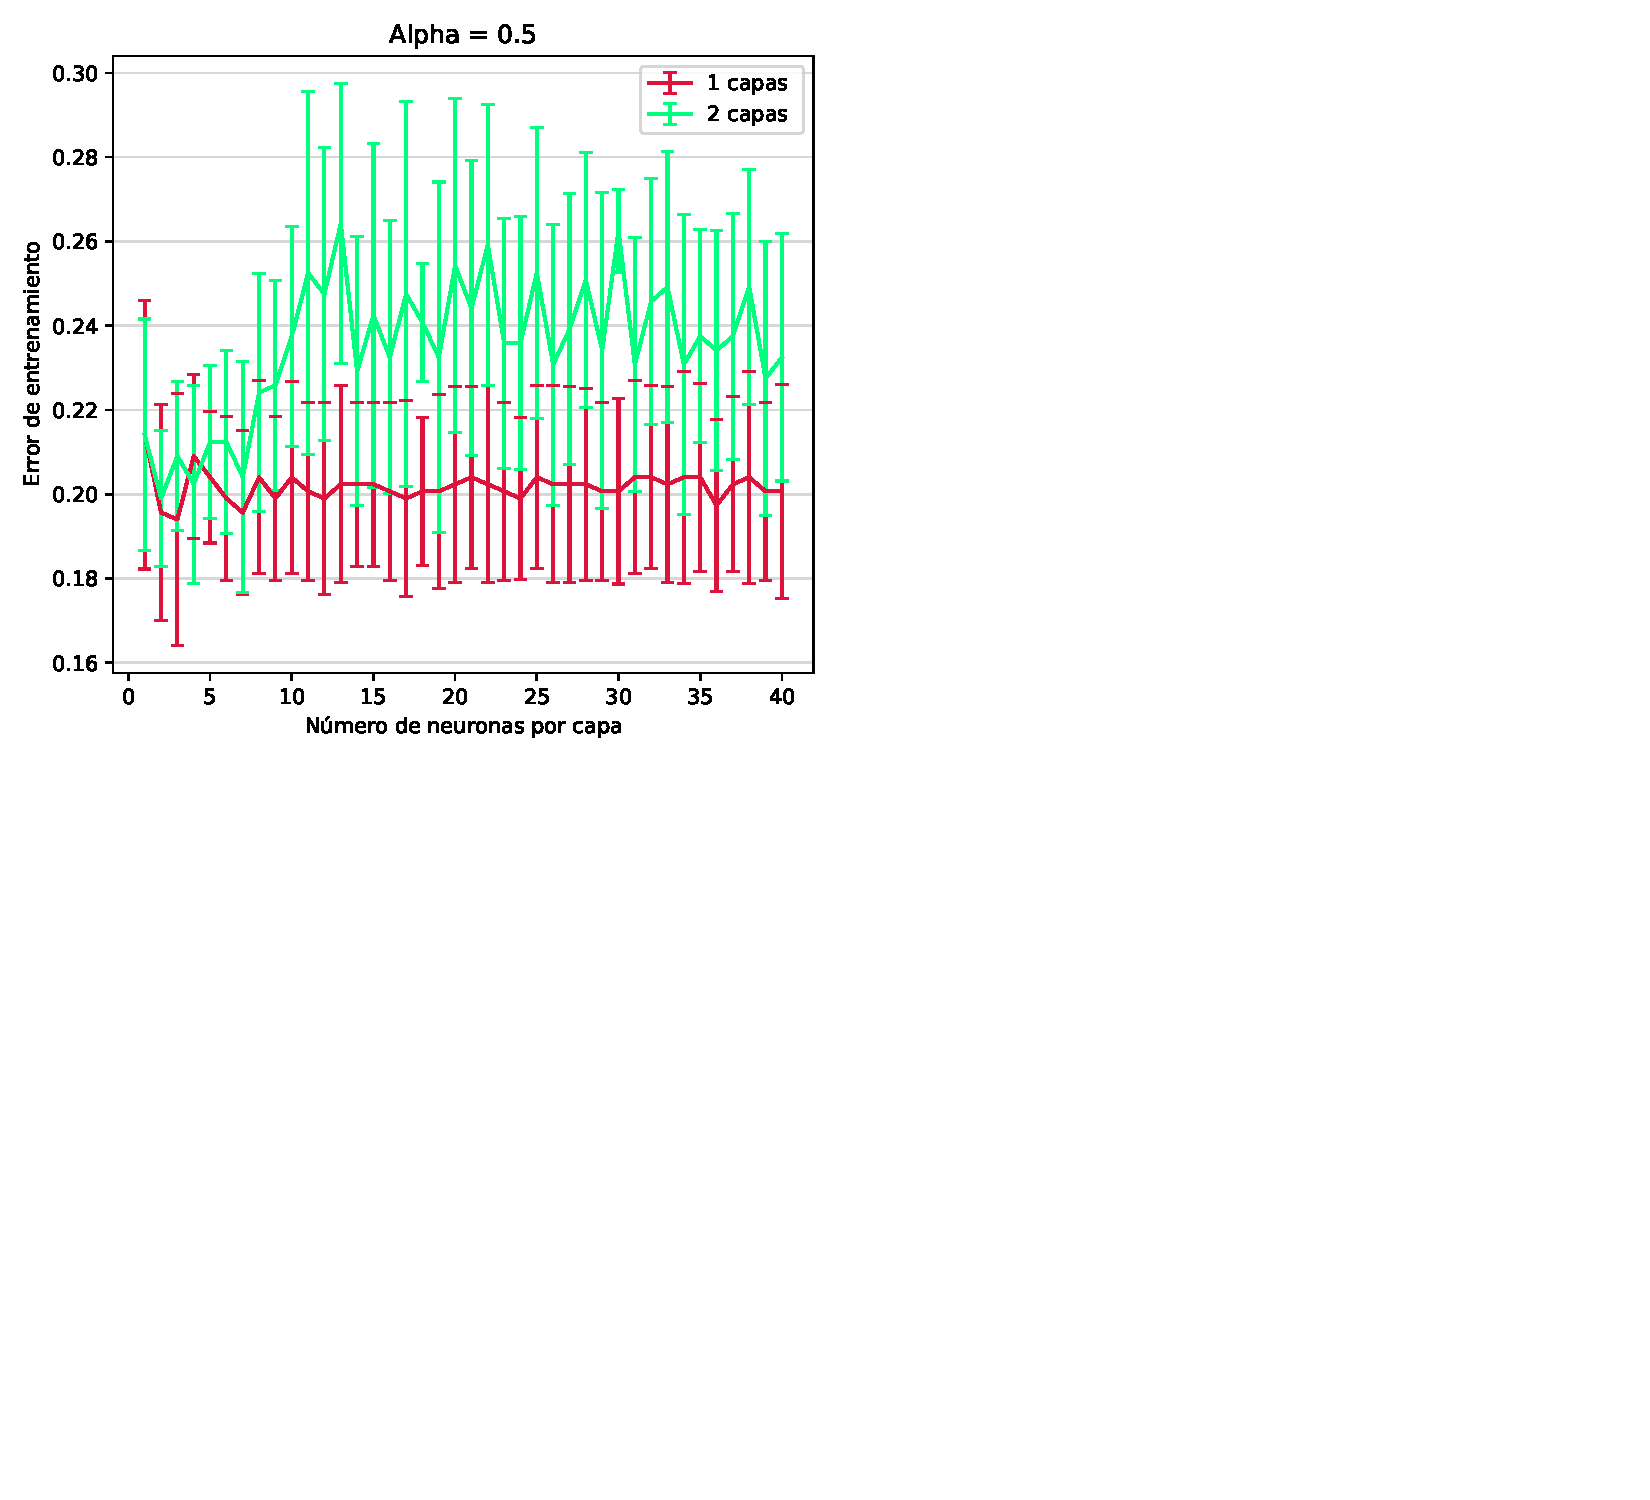
\includegraphics[width=0.8\textwidth]{fotos/ej2_1.pdf}
    \caption{Ejercicio 2: error de validación cruzada en datos de validación.}
    \end{figure}
    \item \textbf{Error de test para los hiperparámetros de validación cruzada:} $\Delta = 0.2$, \\ $\text{param\_hidden\_layer\_sizes} = (3,)$, $\text{param\_alpha} = 0.5$.
    \begin{figure}[h]
    \centering
    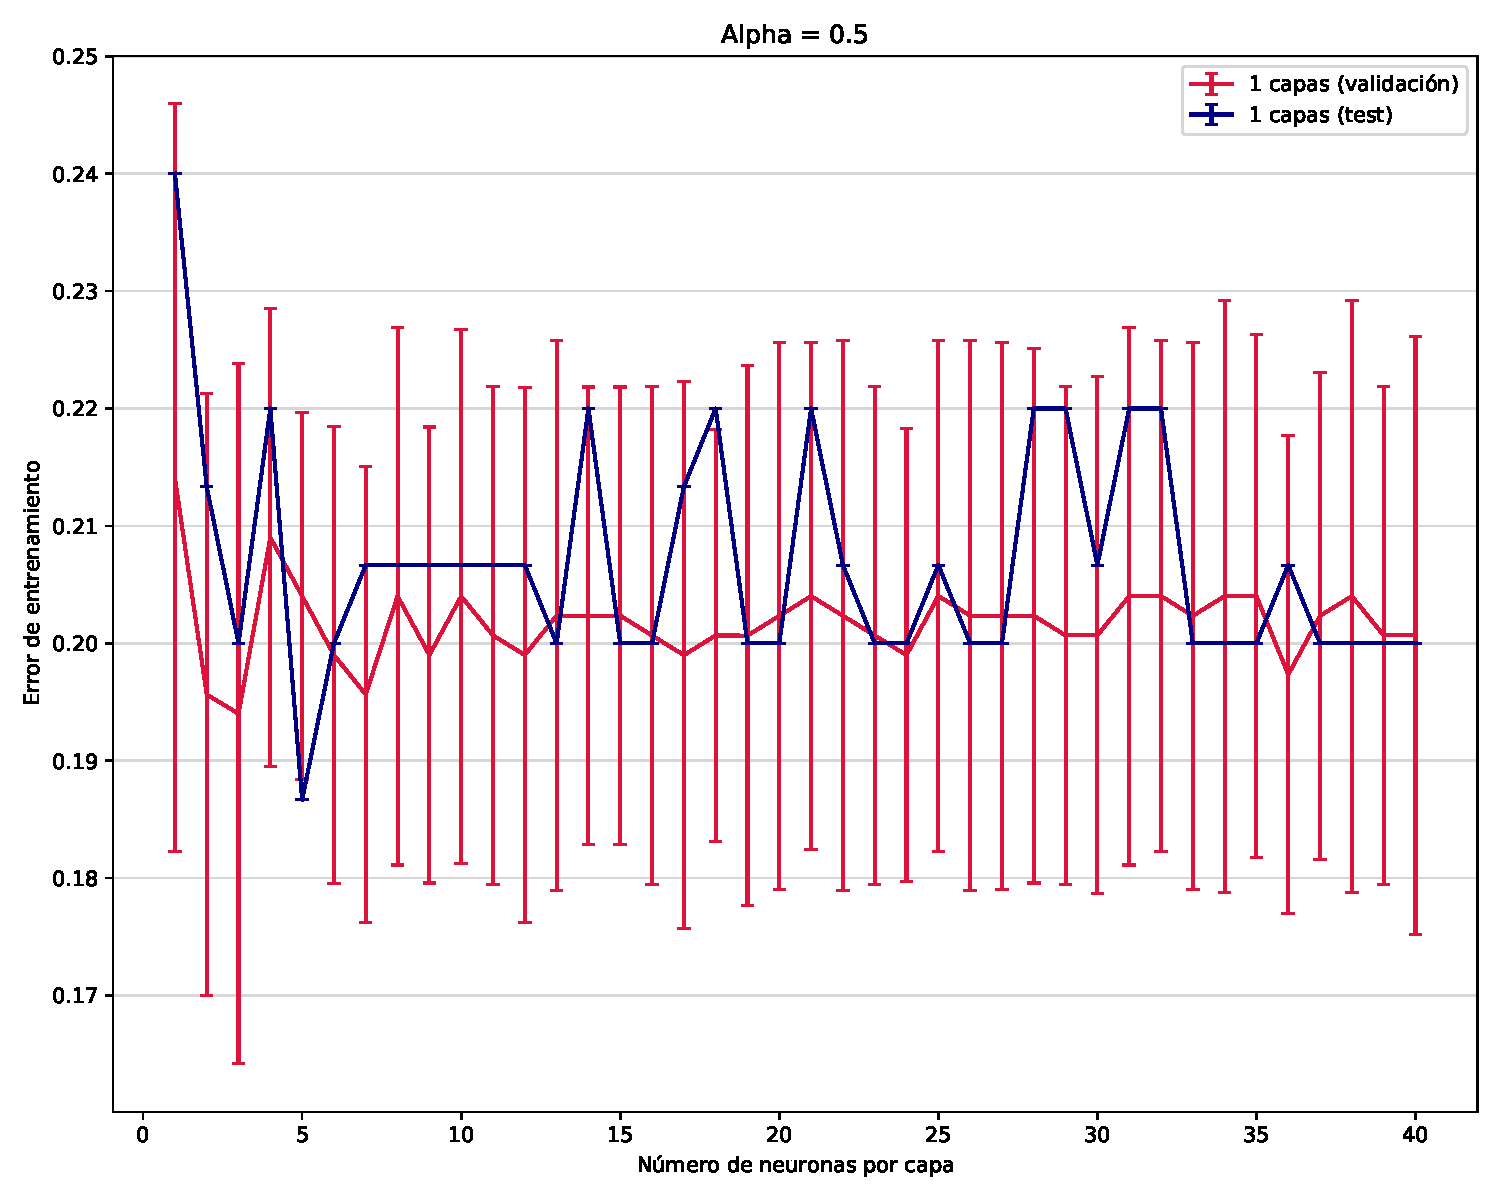
\includegraphics[width=0.8\textwidth]{fotos/ej2_2.pdf}
    \caption{Ejercicio 2: error de validación cruzada en datos de validación frente al mismo error en datos de test.}
    \end{figure}
\end{itemize}


\subsubsection*{Ejercicio 3}

\begin{itemize}
    \item \textbf{Menor error de validación cruzada, su desviación estándar y valor de los hiperparámetros:} $\text{MSE} = 0.479828$, $\sigma = 0.122977$, $\text{param\_hidden\_layer\_sizes} = (32, 32, 32)$, $\text{param\_alpha} = 0.1$.
    \begin{figure}[h]
    \centering
    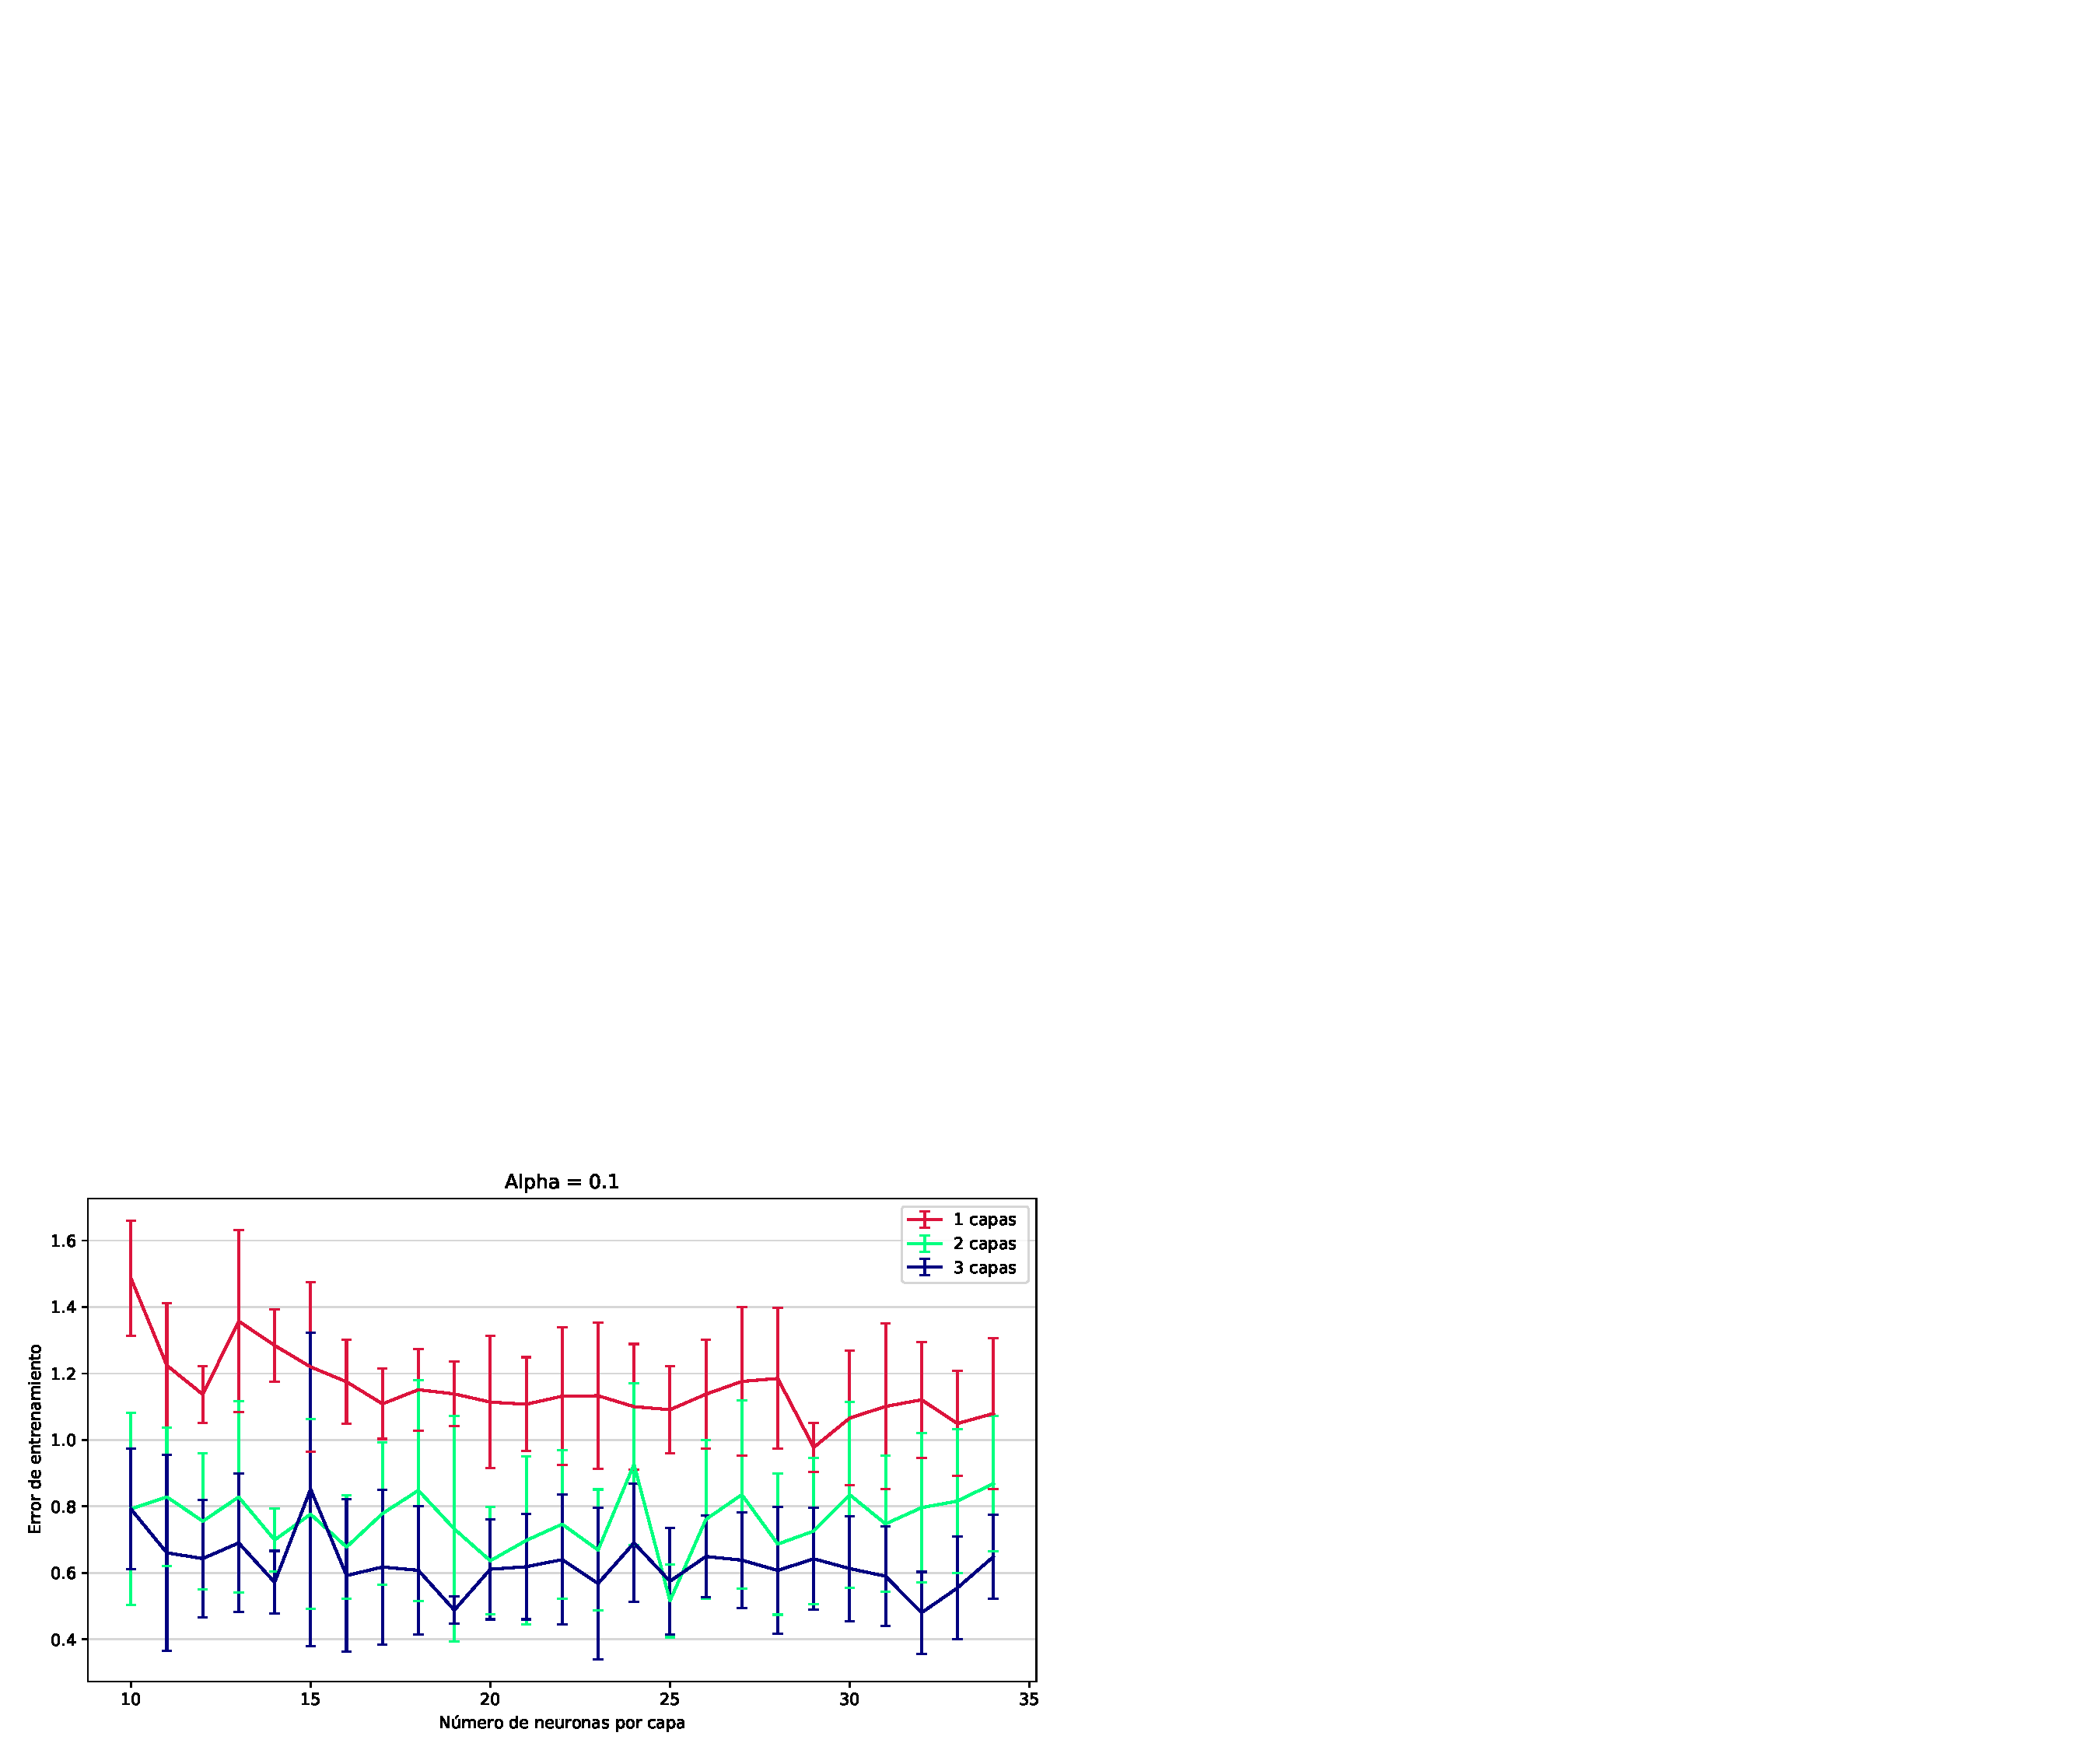
\includegraphics[width=0.8\textwidth]{fotos/ej3_1.pdf}
    \caption{Ejercicio 3: error de validación cruzada en datos de validación.}
    \end{figure}
    \item \textbf{Error de test para los hiperparámetros de validación cruzada:} $\text{MSE} = 0.493655$, \\ $\text{param\_hidden\_layer\_sizes} = (32, 32, 32)$, $\text{param\_alpha} = 0.1$.
    \begin{figure}[h]
    \centering
    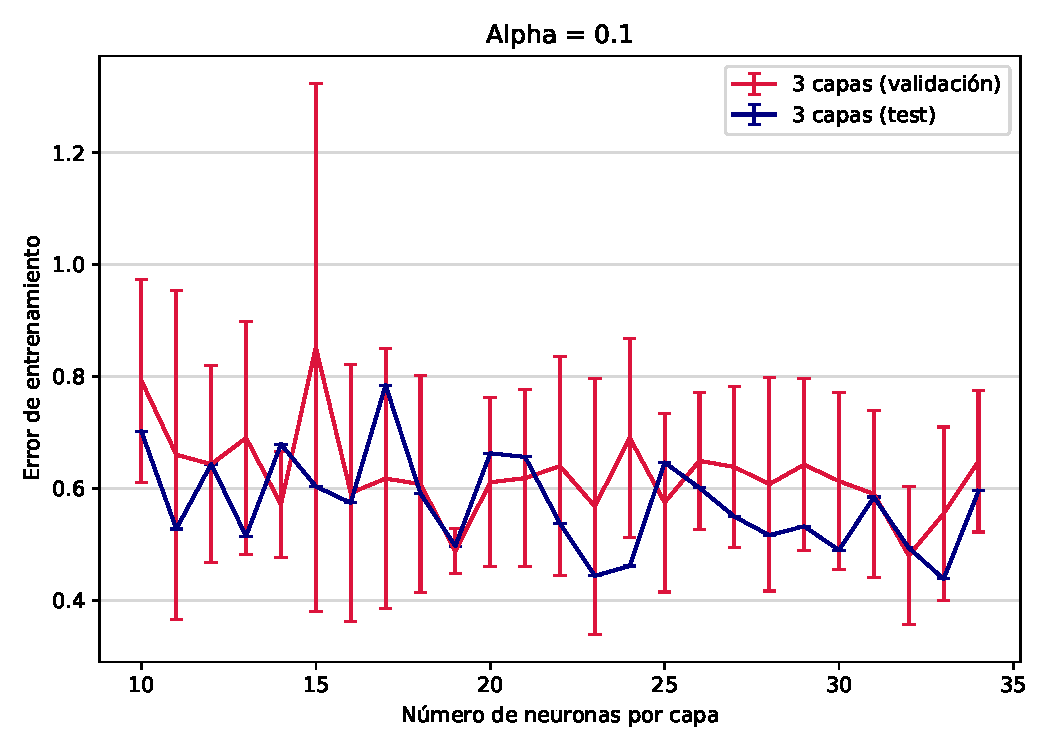
\includegraphics[width=0.8\textwidth]{fotos/ej3_2.pdf}
    \caption{Ejercicio 3: error de validación cruzada en datos de validación frente al mismo error en datos de test.}
    \end{figure}
\end{itemize}


\end{document}
